% -*-coding: utf-8 -*-
\defaultfont
\BiChapter{水下绳驱机械臂运动学建模}{Update Record of the Thesis Model}
\label{Updatelog}


\BiSection{引言}{Introduction}


水下绳驱机械臂虽然在缩减体积方面表现出色，但绳索传动的固有特性不可避免地带
来了强烈的关节运动耦合。加之水下作业极度依赖平稳的操作以减少流体扰动。为
计算这些运动关系，本章从运动学建模切
入。首先利用改进 D-H 法建立正运动学模型，通过数值迭代处理逆解，并推
导得出电机驱动空间到关节空间的映射矩阵。在确立模型后，针对作业的平滑性需求
，分别在关节空间引入了五次多项式过渡，并在笛卡尔空间实现了直线与圆弧的路径
插补。最终的 MATLAB 数值仿真结果验证了算法的计算精度，也为后文控制系统
的软硬件代码编写提供了理论基础。
\BiSection{正运动学建模}{Introduction}
下面将对本文设计的机械臂进行正运动学建模。
为准确描述末端执行器在工作空间中的位置与姿态，
本文选用改进 D-H 参数法建立各关节连杆坐标系。
为后续微分运动分析与实时控制提供模型基础。
\BiSubsection{改进 D-H 法}{Necessary to Use Templates？}
在串联机械臂的运动学分析领域，由 Denavit 和 Hartenberg 提出的 D-H 法是一种广泛应用的标准化求解方法. 该方法的核心在于利用连杆参数描述机构的几何运动关系. 为了克服传统 D-H 法在处理树状构型或基座坐标系定义时的局限性，本文采用改进 D-H 法 进行建模。

(1)改进DH 坐标系建立原则

改进DH 法与传统 D-H 法的主要区别在于坐标系固定位置的不同：改进DH 法将坐标系 $\{i\}$ 固定在连杆 $i$ 的近端. 这种定义方式使得连杆 $i$ 的几何参数与其编号更加一致. 坐标系间的位姿变换由以下四个参数确定：

连杆长度 $a_{i-1}$：沿 $x_{i-1}$ 轴，从 $z_{i-1}$ 轴到 $z_i$ 轴的距离 ；

连杆转角 $\alpha_{i-1}$：绕 $x_{i-1}$ 轴，从 $z_{i-1}$ 轴旋转至 $z_i$ 轴的角度 ；

连杆偏距 $d_i$：沿 $z_i$ 轴，从 $x_{i-1}$ 轴到 $x_i$ 轴的距离 ；

关节角 $\theta_i$：绕 $z_i$ 轴，从 $x_{i-1}$ 轴旋转至 $x_i$ 轴的角度 。

\begin{figure}[H] % htbp代表图片插入位置的设置
  \centering %图片居中
  %添加图片；[]中为可选参数，可以设置图片的宽高；{}中为图片的相对位置
  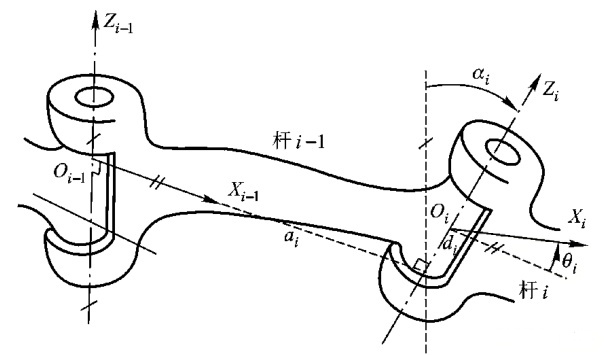
\includegraphics[width = 0.55\textwidth]{figures/DH(1).png}
  \caption{改进DH示意图} % 图片标题
  \label{pic24} % 图片标签      
  \vspace{-0.5cm}
  \end{figure}


(2)齐次变换矩阵推导

根据改进DH法的参数定义，从坐标系 $\{i-1\}$ 到相邻坐标系 $\{i\}$ 的齐次变换矩阵 ${}^{i-1}_{i}T$ 可由绕 $x$ 轴的旋转与平移变换、以及绕 $z$ 轴的旋转与平移变换复合而成. 其数学表达式如下：
\begin{equation}
    \begin{aligned}
        {}^{i-1}_{i}T &= Rot(x_{i-1}, \alpha_{i-1}) \cdot Trans(x_{i-1}, a_{i-1}) \cdot Rot(z_i, \theta_i) \cdot Trans(z_i, d_i) \\
        &= \begin{bmatrix} 
        \cos\theta_i & -\sin\theta_i & 0 & a_{i-1} \\ 
        \sin\theta_i\cos\alpha_{i-1} & \cos\theta_i\cos\alpha_{i-1} & -\sin\alpha_{i-1} & -d_i\sin\alpha_{i-1} \\ 
        \sin\theta_i\sin\alpha_{i-1} & \cos\theta_i\sin\alpha_{i-1} & \cos\alpha_{i-1} & d_i\cos\alpha_{i-1} \\ 
        0 & 0 & 0 & 1 
        \end{bmatrix}
    \end{aligned}
    \label{eq:mdh_matrix}
\end{equation}
其中，$i$ 表示第 $i$ 个关节，各参数意义详见前文描述.

(2)系统总变换方程

对于本文研制的三自由度绳驱机械臂，其末端相对于基座坐标系的运动学总变换矩阵可由各关节变换矩阵连乘得到：
\begin{equation}
    {}^{0}_{3}T = {}^{0}_{1}T({q_1}) \cdot {}^{1}_{2}T({q_2}) \cdot {}^{2}_{3}T({q_3})
    \label{eq:total_t}
\end{equation}

在实际水下作业场景中，需考虑机械臂与运载器及末端执行器的坐标转换 ：

\ding{172}末端补偿：末端执行器坐标系相对于腕部坐标系存在固定变换 $E$，则末端相对于基座坐标系的位姿变换为 ${}^{0}_{E}T = {}^{0}_{3}T \cdot E$.

\ding{173}基座补偿：机械臂基座坐标系相对于水下运载器坐标系存在固定变换 $Z$，则末端执行器相对于运载器参照坐标系的最终变换矩阵为：


\begin{equation}
    {}^{V}_{E}T = Z \cdot {}^{0}_{3}T \cdot E
    \label{eq:final_t}
\end{equation}

通过上述 改进DH 运动学模型，能够准确解算出机械臂末端执行器在空间中的位置与姿态，为后续的轨迹规划与控制打下基础.

\subsection{机械臂 D-H 参数表}
水下绳驱机械臂由三个转动关节组成，依其与运载器基座的连接远近，依次定义为肩关节、肘关节及腕关节。如图 \ref{pic32} 所示，
\begin{figure}[H] % htbp代表图片插入位置的设置
  \centering %图片居中
  %添加图片；[]中为可选参数，可以设置图片的宽高；{}中为图片的相对位置
  
\includegraphics[width = 0.5\textwidth]{05071}
  \caption{机械臂各关节} % 图片标题
  \vspace{-0.5cm}
  \label{pic32} % 图片标签
  \end{figure}
肘关节 2 采用特殊的关联双铰链滚动机构如图\ref{pic33}。
\vspace{-0.5cm}
\begin{figure}[H] % htbp代表图片插入位置的设置
  \centering %图片居中
  %添加图片；[]中为可选参数，可以设置图片的宽高；{}中为图片的相对位置
  
\includegraphics[width = 0.4\textwidth]{双铰链134}
  \caption{双铰链示意图} % 图片标题
  \label{pic33} % 图片标签
  \vspace{-0.5cm}
  \end{figure}
为了描述该关节运动，杆 $L_{2b}$ 相对于杆 $L_{2a}$ 的旋转角度为 $\theta_{2a}$，杆 $L_3$ 相对于杆 $L_{2b}$ 的旋转角度为 $\theta_{2b}$。定义关节 2 的转角为：
\begin{equation}
    \theta_2 = 180^\circ-\theta_{2a} - \theta_{2b}
\end{equation}
其中，由于双铰链结构的对称约束，满足 $\theta_{2a} = \theta_{2b}$。



坐标系建立与描述

为了精确描述机械臂的位姿并便于之后分析，本文根据机械臂的物理结构建立了一系列局部坐标系。所有坐标系均为右手坐标系，且规定 $Z$ 轴正方向垂直向下。各坐标系定义如下：

\ding{172}坐标系 $\{1\}$ (基准坐标系)：原点位于密封仓上舱盖中心，作为整个机械臂运动链的起始参考点。

\ding{173}坐标系 $\{2\}$ (肩关节坐标系)：原点位于肩关节旋转中心，其位置相对于密封仓质心存在安装偏置。

\ding{174}坐标系 $\{3\}$ 与 $\{4\}$ (肘部双铰链坐标系)：针对绳驱机械臂特有的双铰链结构，分别在两个铰链的几何中点建立坐标系，用以描述肘部复杂的非线性运动特征。

\ding{175}坐标系 $\{5\}$ (腕关节坐标系)：原点位于腕关节俯仰与偏航轴线的交汇中点。

\ding{176}坐标系 $\{6\}$ (末端执行器坐标系)：原点位于手爪几何中心，描述末端空间位姿。


图\ref{pic34}为各坐标系在机械臂模型上的具体位置。

\begin{figure}[H] % htbp代表图片插入位置的设置
    \centering %图片居中
    %添加图片；[]中为可选参数，可以设置图片的宽高；{}中为图片的相对位置
    
\includegraphics[width = 0.6\textwidth]{坐标系}
    \caption{坐标系示意图} % 图片标题
    \vspace{-0.5cm}
    \label{pic34} % 图片标签
    \end{figure}

    考虑到水下复杂环境作业的安全需求及绳驱机械臂物理结构的固有约束，
    本文对各活动关节的运动范围进行了严格限定：
    

    （1）肩关节 $q_1$：其角度范围设定为 $[-\pi/2, \pi/2]$。确保机械臂前向作业视野宽阔。

    （2）肘关节 $q_2$：受限于绳驱双铰链机构的耦合特性，$q_2$ 同时驱动两个相邻的转动副实现同步俯仰，其运动范围限定在 $[0, \pi/2]$ 以保证传动张力的稳定性。

    （3）腕关节 $q_3$：其角度范围设定为 $[0, \pi]$ ，增强末端手爪在受限空间内的灵活性。


综上所述，机械臂改进 D-H 参数如表 \ref{tab:dh_params_with_limits} 所示。

% \begin{table}[htbp]
%     \centering
%     \caption{水下绳驱机械臂改进 DH 参数及关节运动范围}
%     \label{tab:dh_params_with_limits}
%     \begin{tabular}{ccccccc}
%     \toprule
%     连杆 $i$ & 物理位置 & $\alpha_{i-1}$ (rad) & $a_{i-1}$ (m) & $d_i$ (m) & $\theta_i$ (rad) & 运动范围 (rad) \\ \midrule
%     1 & 密封仓 $\to$ 肩 & 0 & 0.13500 & 0.09130 & $q_1$ & $[-\pi/2, \pi/2]$ \\
%     2 & 肩 $\to$ 肘 I & $-\pi/2$ & 0.13500 & 0 & $-q_2$ & $[0, \pi/2]$ \\
%     3 & 肘 I $\to$ 肘 II & 0 & 0.08000 & 0 & $-q_2 + 0.06385$ & (联动关节) \\
%     4 & 肘 II $\to$ 腕 & 0 & 0.43881 & 0 & $q_3 - 3.00540$ & $[0, \pi]$ \\
%     5 & 腕 $\to$ 手爪 & $-\pi/2$ & 0.12286 & 0.02214 & 0 & (固定) \\ \bottomrule
%     \end{tabular}
%     \end{table}
\begin{table}[htbp]
    \centering
    \caption{水下绳驱机械臂改进 DH 参数及关节运动范围}
    \label{tab:dh_params_with_limits}
    \begin{tabular}{ccccccc}
    \toprule[2pt]   % 上粗线加粗
    连杆 $i$ & 物理位置 & $\alpha_{i-1}$ (rad) & $a_{i-1}$ (m) & $d_i$ (m) & $\theta_i$ (rad) & 运动范围 (rad) \\
    \midrule
    1 & 密封仓 $\to$ 肩 & 0 & 0.13500 & 0.09130 & $q_1$ & $[-\pi/2, \pi/2]$ \\
    2 & 肩 $\to$ 肘 I & $-\pi/2$ & 0.13500 & 0 & $-q_2$ & $[0, \pi/2]$ \\
    3 & 肘 I $\to$ 肘 II & 0 & 0.08000 & 0 & $-q_2 + 0.06385$ & (联动关节) \\
    4 & 肘 II $\to$ 腕 & 0 & 0.43881 & 0 & $q_3 - 3.00540$ & $[0, \pi]$ \\
    5 & 腕 $\to$ 手爪 & $-\pi/2$ & 0.12286 & 0.02214 & 0 & (固定) \\
    \bottomrule[2pt] % 下粗线加粗
    \end{tabular}
\end{table}




% \BiSection{正运动学建模 }{Introduction}

\subsection{系统总变换方程}

% \begin{equation}
% {}^{i-1}_{i}T = \begin{bmatrix} 
% \cos\theta_i & -\sin\theta_i & 0 & a_{i-1} \\ 
% \sin\theta_i\cos\alpha_{i-1} & \cos\theta_i\cos\alpha_{i-1} & -\sin\alpha_{i-1} & -d_i\sin\alpha_{i-1} \\ 
% \sin\theta_i\sin\alpha_{i-1} & \cos\theta_i\sin\alpha_{i-1} & \cos\alpha_{i-1} & d_i\cos\alpha_{i-1} \\ 
% 0 & 0 & 0 & 1 
% \end{bmatrix}
% \end{equation}
本文采用改进 D-H 法对机械臂进行运动学建模。相邻坐标系 $\{i-1\}$ 到 $\{i\}$ 
之间的齐次变换矩阵通用表达式如式 \ref{eq:mdh_matrix} 所示。根据表 
\ref{tab:dh_params_with_limits} 所列的机械臂结构参数，将各关节变量代入
该通用矩阵中，即可求得相邻连杆间的位姿变换关系。设
水下运载器坐标系为 $\{V\}$，机械臂基座坐标系相对于运载器的安装变换
矩阵为 $Z$，则作业末端执行器在运载器坐标系下的总变换矩阵 ${}^{V}_{E}T$ 
可表示为：
\begin{equation}
    {}^{V}_{E}T = Z \cdot {}^{0}_{1}T({q_1}) \cdot {}^{1}_{2}T({q_2}) \cdot {}^{2}_{3}T({q_2}) \cdot {}^{3}_{4}T({q_3})\cdot E
    \label{e31}
\end{equation}
将各关节之间的变换矩阵带入公式\ref{e31}中，得机械臂位置变换矩阵为:
\begin{equation}
    {}^{V}_{E}T = \begin{bmatrix}
    n_x & o_x & a_x & P_x \\
    n_y & o_y & a_y & P_y \\
    n_z & o_z & a_z & P_z \\
    0 & 0 & 0 & 1
    \end{bmatrix}
    \label{e32}
    \end{equation}
    其中， $\theta_{L} = 2q_2 - 0.06385$,
$\Phi = 2q_2 - q_3 + 2.94155$,
$c_1 = \cos q_1, s_1 = \sin q_1, C_{\Phi} = \cos \Phi, S_{\Phi} = \sin \Phi$

    将中间变量代入式\ref{e32}有：

    (1) 姿态矩阵分量
    \begin{equation}
      \left\{\begin{array}{c}
      n_x = c_1 C_{\Phi} \\
      n_y = s_1 C_{\Phi} \\
      n_z = S_{\Phi}\\
      o_x = s_1 \\
      o_y = -c_1 \\
      o_z = 0\\
      a_x = c_1 S_{\Phi} \\
      a_y = s_1 S_{\Phi} \\
      a_z = -C_{\Phi}
      \end{array}\right.
    \end{equation}

    (2) 位置矢量分量
    \begin{equation}
        \left\{\begin{array}{c}
        P_x = Z_x + c_1 \left[ a_0 + a_1 + a_2 \cos q_2 + a_3 \cos \theta_L + a_4 C_{\Phi} + d_5 S_{\Phi} \right] \\
        P_y = Zy + s_1 \left[ a_0 + a_1 + a_2 \cos q_2 + a_3 \cos \theta_L + a_4 C_{\Phi} + d_5 S_{\Phi} \right] \\
        P_z = Z_z + d_1 + a_2 \sin q_2 + a_3 \sin \theta_L - a_4 S_{\Phi} + d_5 C_{\Phi}
        \end{array}\right.
    \end{equation}
    其中，各几何常数取值如下：$a_0=0.135, a_1=0.135, a_2=0.08, a_3=0.43881, a_4=0.12286, d_1=0.0913, d_5=0.02214$。
    
    由上述计算可得绳驱机械臂搭载的手爪位置相对于运载器的位置矩阵如下：
    \begin{equation}
        P = \begin{bmatrix}
            X \\
            Y \\
            Z \\
        \end{bmatrix}=  \begin{bmatrix}
                        Z_x + c_1 \left[ a_0 + a_1 + a_2 \cos q_2 + a_3 \cos \theta_L + a_4 C_{\Phi} + d_5 S_{\Phi} \right] \\
                        Z_y + s_1 \left[ a_0 + a_1 + a_2 \cos q_2 + a_3 \cos \theta_L + a_4 C_{\Phi} + d_5 S_{\Phi} \right] \\
                        Z_z + d_1 + a_2 \sin q_2 + a_3 \sin \theta_L - a_4 S_{\Phi} + d_5 C_{\Phi}
                        \end{bmatrix}
        \end{equation}

    \BiSection{逆运动学分析}{Introduction}
    逆运动学的核心任务是根据末端执行器的目标位置和姿态，反向求解出各关节所需的物理转角，这也是实现机械臂轨迹跟踪与底层控制的前提。

    求解方法主要分为解析法与数值法两大类。其中，解析法通过代数消元或几何推
    导直接求得关节解。其主要优势在于计算效率极高、无原理误差，但往往要求机械臂
    结构满足一定条件。
    
    相比之下，数值解法则通常借助雅可比矩阵，利用目标位姿与当前实际位姿的差值
    构建误差函数，通过迭代算法逐步逼近真实解。鉴于本文设计的绳驱机械臂引入了
    双铰链等特殊结构。若强行推导解析解，过程极其繁琐。因此，为并保证系统在的
    稳定性，本文最终选用
    数值解法对该绳驱机械臂进行逆运动学求解。
    \subsection{基于雅可比矩阵的简单迭代求解}
    在已知机械手爪期望目标位置 $\boldsymbol{P}_{target} \in \mathbb{R}^{3}$ 的情况下，本文采用经典的牛顿-拉夫逊迭代法进行数值逼近。
    
    设第 $k$ 次迭代的关节变量矢量为 $\boldsymbol{q}_k = [q_1, q_2, q_3]^T$，通过正运动学模型可计算出当前的末端执行器位置 $\boldsymbol{P}(\boldsymbol{q}_k)$。定义位置误差矢量为：
    \begin{equation}
        \boldsymbol{e}_k = \boldsymbol{P}_{target} - \boldsymbol{P}(\boldsymbol{q}_k)
    \end{equation}
    
    机械臂的雅可比矩阵 $\boldsymbol{J}(\boldsymbol{q})$ 反映了关节空间微小变化对笛卡尔空间位姿的线性映射关系，即 $\Delta \boldsymbol{P} \approx \boldsymbol{J} \Delta \boldsymbol{q}$。
    本文采用解析求导法构造 $3 \times 3$ 位置雅可比矩阵：
    \begin{equation}
    \boldsymbol{J}(\boldsymbol{q}) = \begin{bmatrix}
    \frac{\partial P_x}{\partial q_1} & \frac{\partial P_x}{\partial q_2} & \frac{\partial P_x}{\partial q_3} \\
    \frac{\partial P_y}{\partial q_1} & \frac{\partial P_y}{\partial q_2} & \frac{\partial P_y}{\partial q_3} \\
    \frac{\partial P_z}{\partial q_1} & \frac{\partial P_z}{\partial q_2} & \frac{\partial P_z}{\partial q_3}
    \end{bmatrix}
    \end{equation}

    利用伪逆矩阵（Pseudo-inverse）可以得到关节角的迭代更新律：
    \begin{equation}
        \boldsymbol{q}_{k+1} = \boldsymbol{q}_k + \boldsymbol{J}^{\dagger}(\boldsymbol{q}_k) \boldsymbol{e}_k
    \end{equation}
    其中，$\boldsymbol{J}^{\dagger} = \boldsymbol{J}^T (\boldsymbol{J} \boldsymbol{J}^T)^{-1}$ 为雅可比矩阵的伪逆。通过不断重复上述更新过程，当位置误差范数 $\|\boldsymbol{e}_k\|$ 小于设定的容差阈值 $\epsilon$ 时，迭代终止，输出最终的关节角度。
    
    

\subsection{驱动空间与关节空间关系}
在已知电机输出转角 $\phi_i$ 的前提下，求解机械臂末端位姿的关键在于建立从驱动空间至关节空间的运动转换模型。

在绳驱机构中，各关节由独立电机通过绳索驱动。基于几何推导,
各关节转角与驱动电机转角的关系，具体表达为：
\begin{equation}
  \left\{\begin{array}{c}
  q_1=\frac{R_1}{r_1} \theta_1 \\
  q_2=\frac{2 N\left(D_{\max }-D_{\min }\right)}{\pi r_2} \theta_2 \\
  q_3=\frac{R_3}{r_3} \theta_3
  \end{array}\right.
  \end{equation}


但是，由于系统中存在多组导向轮，且导向轮具有一定半径，机械臂各关节之间将产
生运动耦合，即某一关节的运动会引起后续关节的运动。本节将针对肘关节与腕
关节之间的耦合现象进行详细阐述。

(1)肘关节耦合

肘关节的耦合现象主要发生在肩部导向轮，如图\ref{fig:total_figure32}
如图所示，当肩关节旋转$\theta_1$时，
肘关节的两根驱动绳会伸长和缩短长为$\theta_1R_1$的一个弧长
（绿色为缩短，紫色为伸长），为了保证肘关节不动，
肘关节电机需要在肩关节旋转的方向上旋转$\frac{R_2\theta_1}{r_1}$弧度。
\begin{figure}[htbp]
    \centering
    % 第一张子图
    \begin{minipage}{\textwidth}
        \centering
        \subfigure[肩关节未旋转]{\label{fig32:sub1}
            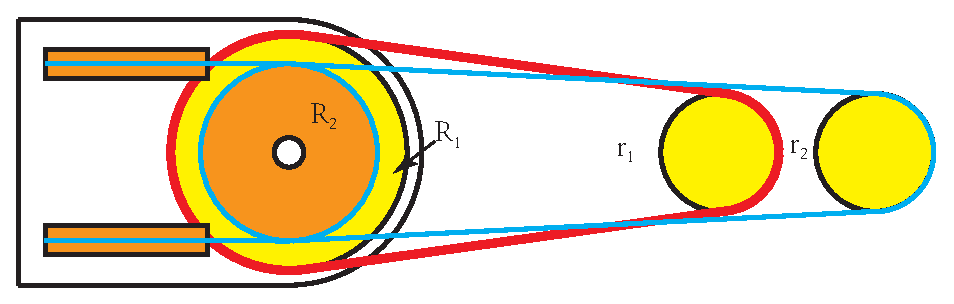
\includegraphics[width =0.6 \textwidth]{figures/耦合1.eps}
        }% 这里写第一张图的英文描述
    \end{minipage}
    % \hfill % 撑开左右间距
    % 第二张子图
    \begin{minipage}{\textwidth}
        \centering
        \subfigure[肩关节旋转$\theta_1$]{\label{fig32:sub2}
            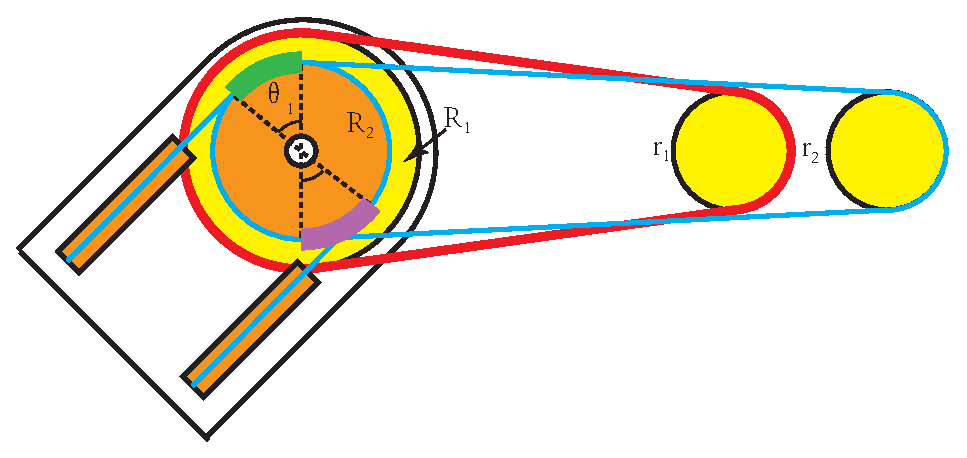
\includegraphics[width = 0.6 \textwidth]{figures/耦合2.eps}
        } % 这里写第二张图的英文描述
             % 第一张子图
            \end{minipage}
    % 中英文总标题

    \caption{肘关节耦合原理}
    \vspace{-0.5cm}
    \label{fig:total_figure32}
  \end{figure}


(2)腕关节耦合

由于腕关节驱动绳也经过肩部导向轮，
所以腕关节也会存在耦合现象且原理和肘关节相同，
同时腕关节驱动绳同时绕过肘部导向轮上方，如图
\ref{fig:total_figure33}，当肘部关节旋转的
时候腕关节驱动绳会同时伸长或缩短，所以肘部导向轮对腕关节无耦合影响，
腕关节电机只需在肩关节旋转的方向上旋转$\frac{R_4\theta_1}{r_3}$弧度。

\begin{figure}[htbp]
    \centering
    % 第一张子图
    \begin{minipage}{\textwidth}
        \centering
        \subfigure[肘关节未旋转]{\label{fig33:sub1}
            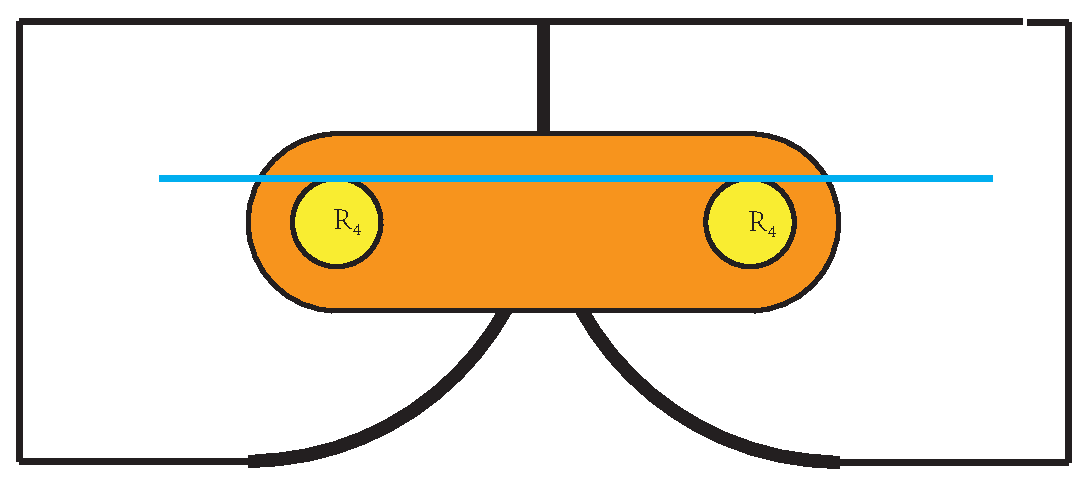
\includegraphics[width =0.4 \textwidth]{figures/腕关节解耦.eps}
        }% 这里写第一张图的英文描述
    \end{minipage}
    % \hfill % 撑开左右间距
    % 第二张子图
    \begin{minipage}{\textwidth}
        \centering
        \subfigure[肘关节旋转$\theta_2$]{\label{fig33:sub2}
            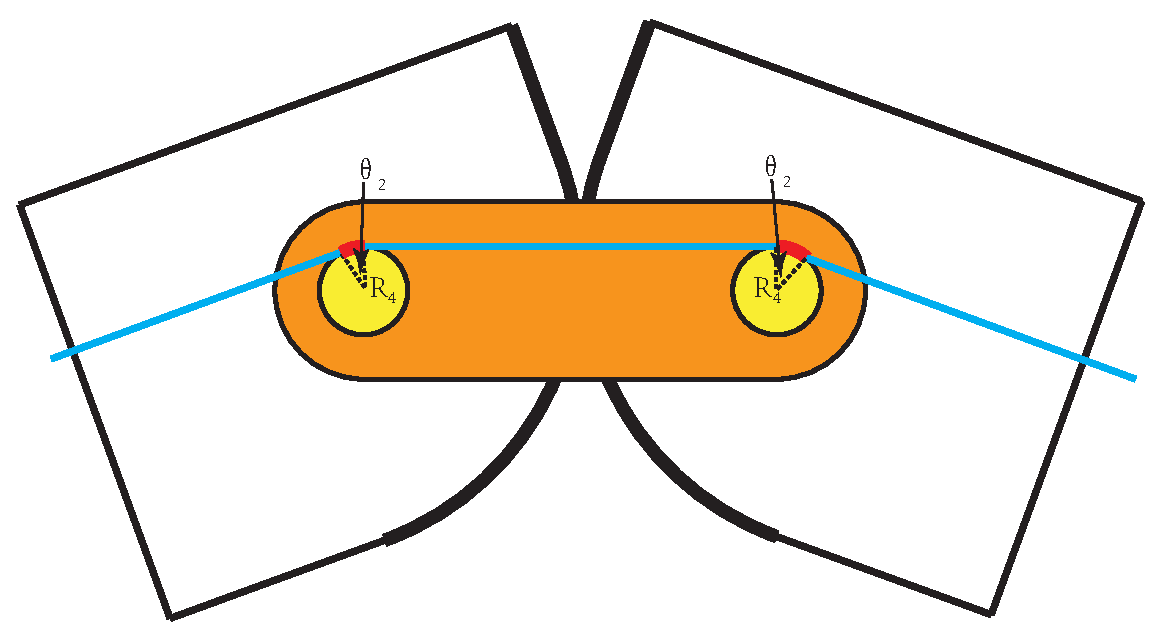
\includegraphics[width = 0.4 \textwidth]{figures/腕关节耦合2.eps}
        } % 这里写第二张图的英文描述
             % 第一张子图
            \end{minipage}
    % 中英文总标题
    \caption{腕关节耦合原理}
    \label{fig:total_figure33}
  \end{figure}
结合几何推导和耦合关系各关节转角与驱动电机转角的关系，具体表达为：
\begin{equation}
    \left\{\begin{array}{c}
    q_1=\frac{R_1}{r_1} \theta_1 \\
    q_2=\frac{2 N\left(D_{\max }-D_{\min }\right)}{\pi r_2} \theta_2+\frac{R_2\theta_1}{r_1} \\
    q_3=\frac{R_3}{r_3} \theta_3+\frac{R_3\theta_1}{r_3}
    \end{array}\right.
    \end{equation}
  

驱动电机转角矢量 $\boldsymbol{\Phi} = [\phi_1, \phi_2, \phi_3]^T$ 与关节角矢量 $\boldsymbol{\Theta} = [\theta_1, \theta_2, \theta_3]^T$ 的线性映射关系可表示为：
\begin{equation}
\begin{bmatrix} \phi_1 \\ \phi_2 \\ \phi_3 \end{bmatrix} = 
\boldsymbol{M}
\begin{bmatrix} \theta_1 \\ \theta_2 \\ \theta_3 \end{bmatrix} =
\begin{bmatrix} 
\frac{R_1}{r_1} & 0 & 0 \\
\frac{R_2}{r_1} & \frac{2 N\left(D_{\max }-D_{\min }\right)}{\pi r_2} \theta_2  & 0 \\
\frac{R_4}{r_3} & 0 & \frac{R_3}{r_3}
\end{bmatrix}
\begin{bmatrix} \theta_1 \\ \theta_2 \\ \theta_3 \end{bmatrix}
\label{eq:mapping_matrix}
\end{equation}
式中，$r_1, r_2, r_3$ 分别为电机端驱动绞盘的半径；$R_1$ 为肩关节驱动绞盘 ；$R_2$，$R_3$ 分别为肘关节和腕关节肩部导向轮半径；$R_4$为腕关节驱动绳肘部导向轮半径；对于肘关节，其传动比受绕线圈数 $N$ 及绕线轴中心距 $D$ 的综合影响。

根据实验样机的实际物理参数，取 $r_1=r_2=r_3=13\text{mm}$，$R_1=32\text{mm}$，$R_2=20\text{mm}$，$R_3=20\text{mm}$，$R_4=15\text{mm}$，$N=4$，$D=28\text{mm}$。将其代入式 \ref{eq:mapping_matrix} 可得传动映射矩阵：
\begin{equation}
\begin{bmatrix} \phi_1 \\ \phi_2 \\ \phi_3 \end{bmatrix} = 
\begin{bmatrix} 
2.46 & 0 & 0 \\
1.53 & 13.53 & 0 \\
1.15 & 0 & 1.54
\end{bmatrix}
\begin{bmatrix} \theta_1 \\ \theta_2 \\ \theta_3 \end{bmatrix}
\end{equation}

该关系为机械臂的精确轨迹规划提供理论依据。通过对耦合关系进行数学建模，得到
驱动电机到关节转角的关系，
控制系统能够根据末端目标位姿反求各个关节角度，通过各个关节角度来反求各驱动电机
的转角，从而提升机械臂的准确性。

\subsection{数值仿真验证}
为了验证上述数值迭代法的有效性，本文基于 MATLAB 编写了逆运动学解算算法，
并进行了一系列仿真实验。
从仿真结果来看，对于工作空间内的目标点，
迭代法能够稳定求解各关节角度，末端位置误差始终控制在 0.005\% 以内。
在多次随机采样测试中，算法均可收敛至误差范围，解未出现发散或跳变。
\begin{figure}[H]
        \centering
        % 第一张子图
        \begin{minipage}{0.45\textwidth}
            \centering
            \subfigure[X:0.6 Y:0.0 Z:0.6]{\label{fig31:sub1}
                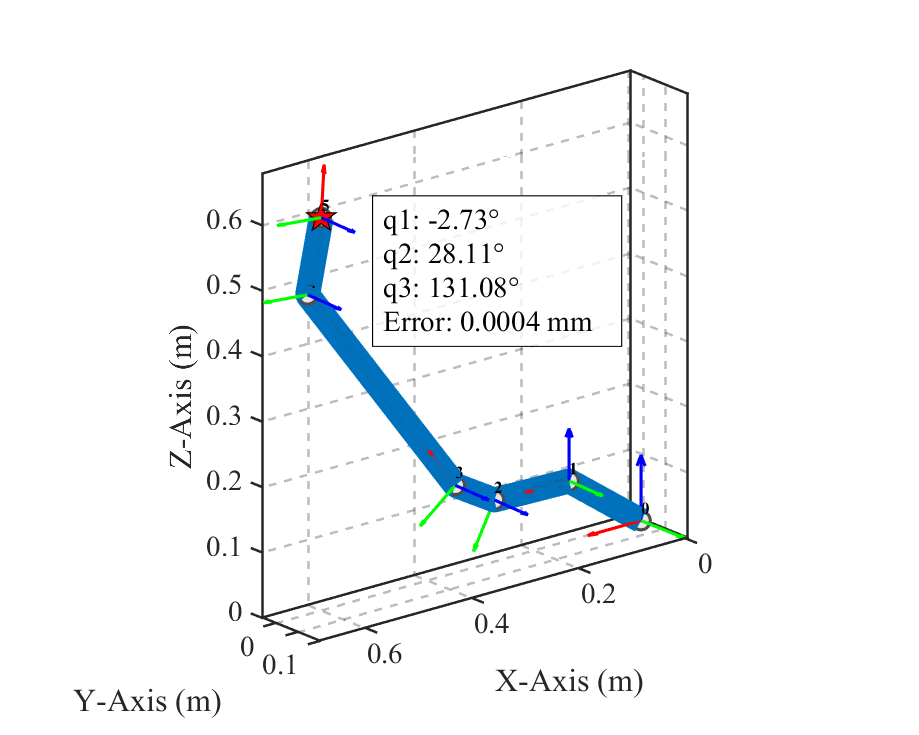
\includegraphics[width =\textwidth]{figures/05606.eps}
            }% 这里写第一张图的英文描述
        \end{minipage}
        % \hfill % 撑开左右间距
        % 第二张子图
        \begin{minipage}{0.45\textwidth}
            \centering
            \subfigure[X:0.6 Y:0.1 Z:0.6]{\label{fig31:sub2}
                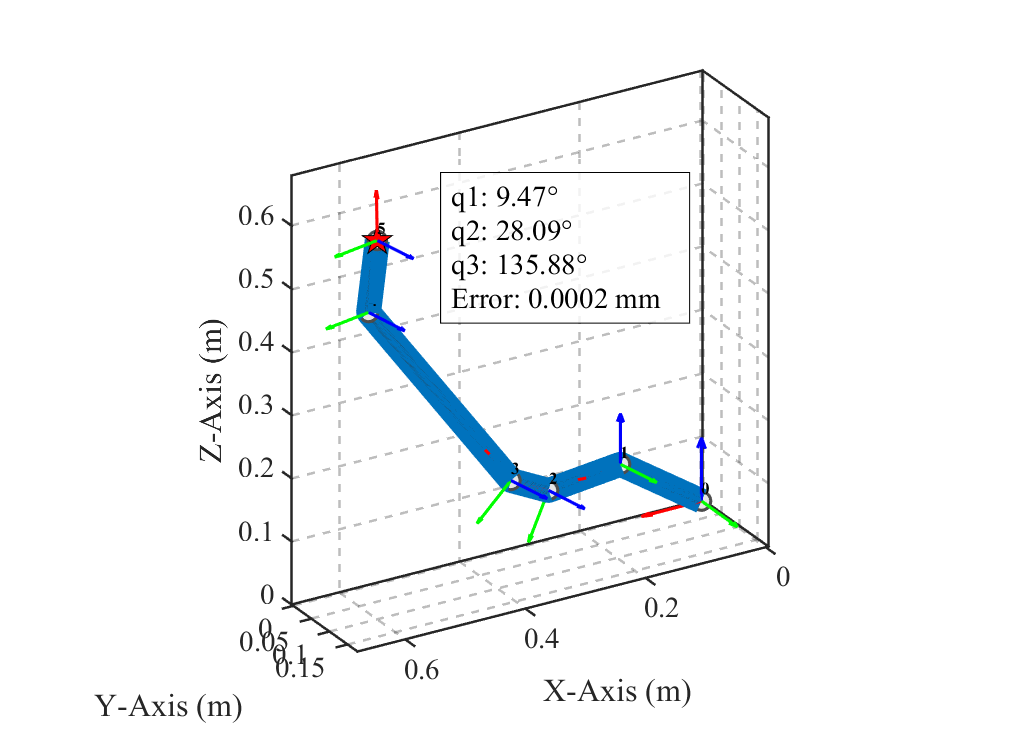
\includegraphics[width =1.1\textwidth]{figures/05616.eps}
            } % 这里写第二张图的英文描述
                 % 第一张子图
                \end{minipage}
        \begin{minipage}{0.45\textwidth}
            \centering
            \subfigure[X:0.7 Y:0.0 Z:0.5]{\label{fig31:sub3}
                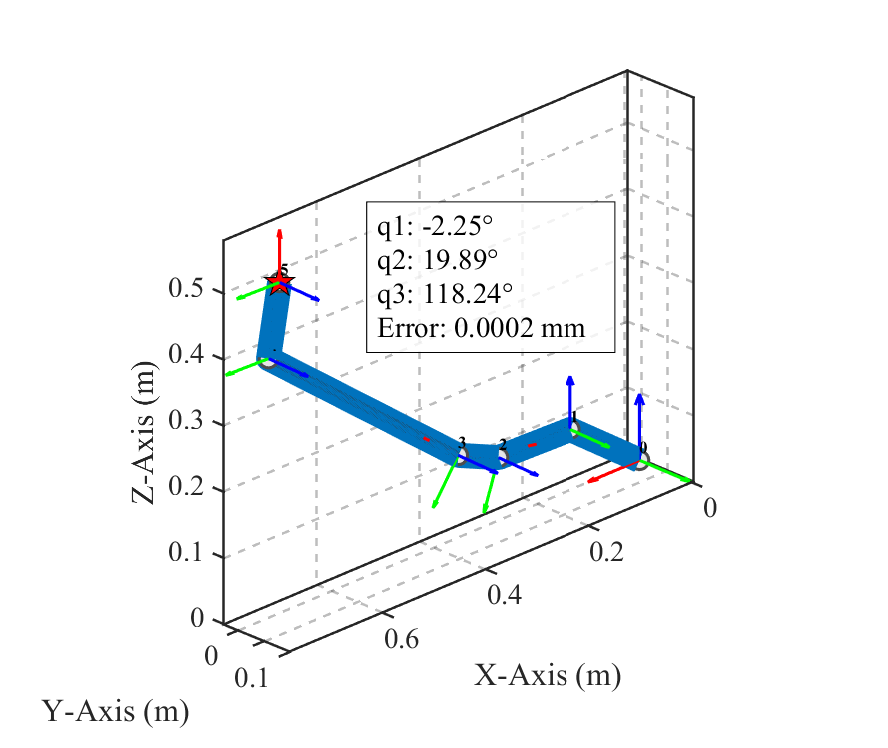
\includegraphics[width =\textwidth]{figures/50705.eps}
            }% 这里写第一张图的英文描述
        \end{minipage}
        % \hfill % 撑开左右间距
        % 第二张子图
        \begin{minipage}{0.45\textwidth}
            \centering
            \subfigure[X:0.7 Y:-0.2 Z:0.5]{\label{fig31:sub4}
                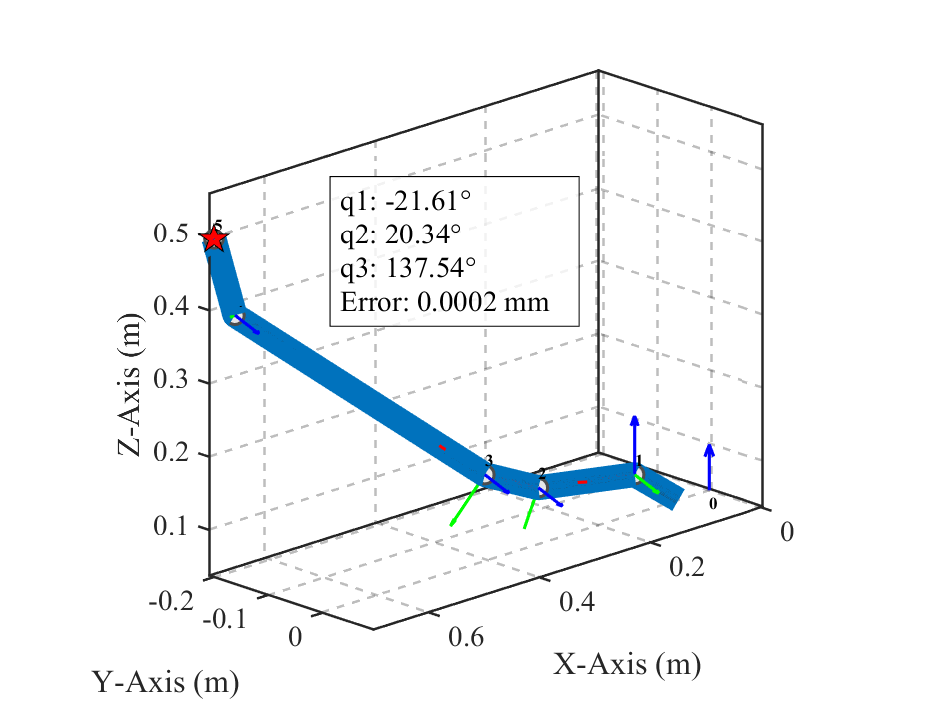
\includegraphics[width = 1.1\textwidth]{figures/05057225.eps}
            } % 这里写第二张图的英文描述
        \end{minipage}
      
        % 中英文总标题
        \caption{部分仿真结果}
        \vspace{-0.5cm}
        \label{fig:total_figure31}
      \end{figure}





      




% \BiSection{水下绳驱机械臂轨迹规划与仿真}{To Template Maintainers}

% \BiSection{引言}{Simple Introduction about This Template}


% 常用的机械臂轨迹规划方法可分为两类：一类是在关节空间中进行规划，用户对选定的插值点上的位姿、
% 速度、加速度给出显式约束（如连续性、光滑性），规划器采用多项式等函数对节点进行插值。该方法
% 计算简单、关节运动平滑，但由于未对末端笛卡尔路径施加直接约束，用户难以预知末端的实际空间轨
% 迹，存在与障碍物碰撞的风险。另一类是在笛卡尔空间中进行规划，用户直接给出末端运动路径的解析
% 表达式（如直线、圆弧），规划器在关节空间或笛卡尔空间中逼近预定路径。该方法能直观控制末端轨
% 迹，便于避障，但需实时求解逆运动学，计算负担较重。

% 本文所研究的水下绳驱机械臂具有三自由度、关节耦合性强、驱动后置等特点，前文已建立其改进 D-H 
% 运动学模型及驱动空间到关节空间的映射关系。为实现机械臂在水下复杂环境中的平稳、精确作业，本
% 章将综合关节空间与笛卡尔空间规划的优势，分别开展基于多项式插值的关节空间轨迹规划与基于直线
% /圆弧插补的笛卡尔空间轨迹规划，并利用 MATLAB 进行数值仿真，对比分析两种方法在末端轨迹精度、
% 关节速度/加速度连续性及计算效率等方面的表现，为后续控制系统设计提供理论依据。

\BiSection{关节空间轨迹规划}{Maintaining Tools Introduction}

关节空间轨迹规划的目标是在给定起始位姿和目标位姿的情况下，通过插值算法生成一系列连续的关节角度、角速度及角加速度序列，从而驱动机械臂完成预定任务。
在水下环境中，为了减小机械臂运动对水体的扰动，轨迹规划需满足连续性和平稳性。
同时为了保证电机不被损坏 需满足关节转角范围、最大角速度及最大角加速度约束。
\BiSubsection{多项式插值规划算法}{Subsubsection}

考虑到水下作业对机械臂运动平稳性的严苛要求，单纯依赖低阶多项式
（例如三次多项式）进行轨迹规划存在明显的工程局限。该算法在启停
瞬间会导致系统的加加速度不连续，进而引发强烈的水体扰动。
为此，本文采用五次多项式来构建关节角度的时间函数，从
根源上平滑加速度曲线，以保障机械臂水下运行的柔顺性。

设关节在 $t=0$ 时刻的初始状态为：位置 $q_0$、速度 $v_0$、加速度 $a_0$；在作业时间 $t=T$ 时刻的末端状态为：位置 $q_f$、速度 $v_f$、加速度 $a_f$。据此可构建关于时间 $t$ 的五次多项式位置函数及其一阶导数（速度方程）和二阶导数（加速度方程）：
\begin{equation}
    \begin{cases}
    q(t) = c_0 + c_1 t + c_2 t^2 + c_3 t^3 + c_4 t^4 + c_5 t^5\\
    \dot{q}(t) = c_1 + 2c_2 t + 3c_3 t^2 + 4c_4 t^3 + 5c_5 t^4\\
    \ddot{q}(t) = 2c_2 + 6c_3 t + 12c_4 t^2 + 20c_5 t^3
    \end{cases}
\end{equation}

将轨迹规划的始末边界条件代入上述方程，可得到如下 $6 \times 6$ 的约束方程组：
\begin{equation}
    \begin{cases}
        q(0) = c_0 = q_0 \\
        \dot{q}(0) = c_1 = v_0 \\
        \ddot{q}(0) = 2c_2 = a_0 \\
        q(T) = c_0 + c_1 T + c_2 T^2 + c_3 T^3 + c_4 T^4 + c_5 T^5 = q_f \\
        \dot{q}(T) = c_1 + 2c_2 T + 3c_3 T^2 + 4c_4 T^3 + 5c_5 T^4 = v_f \\
        \ddot{q}(T) = 2c_2 + 6c_3 T + 12c_4 T^2 + 20c_5 T^3 = a_f
    \end{cases}
\end{equation}

为了便于在计算系统中进行离散化求解，将其转换为矩阵表达形式：

\begin{equation}
    \begin{bmatrix}
        1 & 0 & 0 & 0 & 0 & 0 \\
        0 & 1 & 0 & 0 & 0 & 0 \\
        0 & 0 & 2 & 0 & 0 & 0 \\
        1 & T & T^2 & T^3 & T^4 & T^5 \\
        0 & 1 & 2T & 3T^2 & 4T^3 & 5T^4 \\
        0 & 0 & 2 & 6T & 12T^2 & 20T^3
    \end{bmatrix}
    \begin{bmatrix}
        c_0 \\ c_1 \\ c_2 \\ c_3 \\ c_4 \\ c_5
    \end{bmatrix}
    =
    \begin{bmatrix}
        q_0 \\ v_0 \\ a_0 \\ q_f \\ v_f \\ a_f
    \end{bmatrix}
\end{equation}

通过矩阵求逆及代数消元运算，可解析得出该多项式轨迹方程的全部待定系数：

% \begin{equation}
%     \begin{cases}
%         c_0 = q_0 \\
%         c_1 = v_0 \\
%         c_2 = \frac{a_0}{2} \\
%         c_3 = \frac{20(q_f - q_0) - (8v_f + 12v_0)T - (3a_0 - a_f)T^2}{2T^3} \\
%         c_4 = \frac{-30(q_f - q_0) + (14v_f + 16v_0)T + (3a_0 - 2a_f)T^2}{2T^4} \\
%         c_5 = \frac{12(q_f - q_0) - 6(v_f + v_0)T - (a_0 - a_f)T^2}{2T^5}
%     \end{cases}
% \end{equation}
\begin{equation}
    \begin{cases}
    c_0 = q_0 \\
    c_1 = v_0 \\
    c_2 = \dfrac{a_0}{2}\\
    % \end{cases}
    % \end{equation}
    % \begin{equation*}
    % \begin{cases}
    c_3 = \dfrac{20(q_f - q_0) - (8v_f + 12v_0)T - (3a_0 - a_f)T^2}{2T^3} \\[8pt]
    c_4 = \dfrac{-30(q_f - q_0) + (14v_f + 16v_0)T + (3a_0 - 2a_f)T^2}{2T^4} \\[8pt]
    c_5 = \dfrac{12(q_f - q_0) - 6(v_f + v_0)T - (a_0 - a_f)T^2}{2T^5}
    \end{cases}
    \end{equation}

将上述系数带回原多项式，即可生成给定时间 $T$ 内平滑且满足运动学约束的轨迹。

\BiSubsection{梯形速度规划算法}{Subsubsection}

在水下执行摄像扫描或目标抓取等任务时，常要求机械臂末端保持平稳的匀速运动。此时，梯形速度规划算法具有更高的工程实用性。

梯形速度规划通过分段函数将整个运动周期划分为三个核心区间：匀加速段、匀速作业段与匀减速段。设关节的起始位置为 $q_0$，目标位置为 $q_f$，系统允许的最大运行角速度为 $v_{max}$，最大允许加速度为 $a_{max}$。

若给定的目标路径长度足以支撑系统加速至最高速度，即满足阈值条件 $|q_f - q_0| > \frac{v_{max}^2}{a_{max}}$ 时，系统的加速时间 $t_a$ 及总运行时间 $T$ 定义为：
\begin{equation}
    t_a = \frac{v_{max}}{a_{max}}, \quad T = \frac{|q_f - q_0|}{v_{max}} + t_a
\end{equation}

假设 $q_f > q_0$ 且系统的起止速度均为 $0$，该规划算法在时间轴上速度方程如下：

\textbf{（1）匀加速段 ($0 \le t \le t_a$)}

此阶段机械臂电机输出恒定大扭矩，以最大加速度 $a_{max}$ 启动，其运动方程为：
\begin{equation}
    \begin{cases}
        q(t) = q_0 + \frac{1}{2} a_{max} t^2 \\
        \dot{q}(t) = a_{max} t \\
        \ddot{q}(t) = a_{max}
    \end{cases}
\end{equation}

\textbf{（2）匀速作业段 ($t_a < t \le T - t_a$)}

达到设定巡航速度后，系统加速度降为 $0$，保持 $v_{max}$ 匀速运行以提升作业质量：
\begin{equation}
    \begin{cases}
        q(t) = q_0 + \frac{1}{2} a_{max} t_a^2 + v_{max} (t - t_a) \\
        \dot{q}(t) = v_{max} \\
        \ddot{q}(t) = 0
    \end{cases}
\end{equation}

\textbf{（3）匀减速段 ($T - t_a < t \le T$)}

临近目标点时，机械臂以反向最大加速度 $-a_{max}$ 平滑制动：
\begin{equation}
    \begin{cases}
        q(t) = q_f - \frac{1}{2} a_{max} (T - t)^2 \\
        \dot{q}(t) = v_{max} - a_{max}(t - (T - t_a)) \\
        \ddot{q}(t) = -a_{max}
    \end{cases}
\end{equation}

特别地，在算法设计时需要考虑退化情况。若规划的目标位移过短（即 $|q_f - q_0| \le \frac{v_{max}^2}{a_{max}}$），系统在达到最大设定速度前即需触发减速指令。此时梯形速度曲线退化为三角形速度曲线，算法必须自适应重新计算实际可达的峰值速度 $v'_{max} = \sqrt{|q_f - q_0| a_{max}}$，并将匀速段运行时间置为零以防止位置超调。

\BiSubsection{仿真与结果分析}{Subsubsection}


为了验证本文所提出的五次多项式插值算法与梯形速度规划算法在水下绳驱机械臂关节空间轨迹规划中的
有效性，本章利用 MATLAB 仿真平台进行数值仿真对比。通过分析关节的位置、速度、加速度及加加速度
曲线，评估算法在平滑性、作业效率以及对水下环境影响等方面的表现。

（1）关节规划仿真环境与参数设置

实验设定机械臂某电机从起始角度 $q_0 = 0^\circ$ 运动至目标角度 $q_f = 90^\circ$。为了确保仿真符合工程实际，结合电机的物理性能，设定了最大速度与加速度限制。具体参数如表 \ref{tab:params} 所示。

\begin{table}[htbp]
    \centering
    \caption{关节空间轨迹规划仿真参数}
    \label{tab:params}
    \begin{tabular}{lcc}
    \toprule[1.5pt]
    \textbf{参数名称} & \textbf{符号} & \textbf{设定值} \\
    \midrule
    起始位置  & $q_0$ & $0^\circ$ \\
    目标位置 & $q_f$ & $90^\circ$ \\
    最大允许速度 & $v_{max}$ & $20^\circ/s$ \\
    最大允许加速度  & $a_{max}$ & $10^\circ/s^2$ \\
    仿真步长  & $\Delta t$ & $0.01s$ \\
    \bottomrule[1.5pt]
    \end{tabular}
    \end{table}

    （2）仿真结果分析

    基于上述参数，进行梯形速度规划与五次多项式插值，得到对比曲线如图\ref{fig:total_figure311}所示。
    \begin{figure}[H]
        \centering
        % 第一张子图
        \begin{minipage}{0.45\textwidth}
            \centering
            \subfigure[位置曲线对比]{\label{fig311:sub1}
                \includegraphics[width =0.9\textwidth]{figures/关节1.eps}
            }% 这里写第一张图的英文描述
        \end{minipage}
        % \hfill % 撑开左右间距
        % 第二张子图
        \begin{minipage}{0.45\textwidth}
            \centering
            \subfigure[速度曲线对比]{\label{fig311:sub2}
                \includegraphics[width =0.9\textwidth]{figures/关节2.eps}
            } % 这里写第二张图的英文描述
                 % 第一张子图
                \end{minipage}
        \begin{minipage}{0.45\textwidth}
            \centering
            \subfigure[加速度曲线对比]{\label{fig311:sub3}
                \includegraphics[width =0.9\textwidth]{figures/关节3.eps}
            }% 这里写第一张图的英文描述
        \end{minipage}
        % \hfill % 撑开左右间距
        % 第二张子图
        \begin{minipage}{0.45\textwidth}
            \centering
            \subfigure[Jerk曲线对比]{\label{fig311:sub4}
                \includegraphics[width = 0.9\textwidth]{figures/关节4.eps}
            } % 这里写第二张图的英文描述
        \end{minipage}
        % 中英文总标题
        \caption{对比曲线（实线为五次多项式，虚线为梯形规划）}
        \vspace{-0.5cm}
        \label{fig:total_figure311}
      \end{figure}
    % \begin{figure}[H] % htbp代表图片插入位置的设置
    %     \centering %图片居中
    %     %添加图片；[]中为可选参数，可以设置图片的宽高；{}中为图片的相对位置
    %     
\includegraphics[width = \textwidth]{关节轨迹规划}
    %     \caption{对比曲线} % 图片标题
    %     \label{pic41} % 图片标签
    %     \vspace{-0.5cm}
    % \end{figure}
    结合上述仿真对比曲线，现从位置、速度与加速度、加加速度三个方面对两种规划
    算法的运动学特性进行详细分析：
    
    \ding{172} 位置曲线分析：
    如图\ref{fig:total_figure311}所示，梯形速度规划在中间段为线性增长，而五次多项式轨迹则
    呈现出圆滑的“S”型曲线。
    
    \ding{173} 速度与加速度分析：
    梯形速度规划在加速段和减速段保持恒定的加速度，这虽然缩短了运动时间，但其
    加速度曲线在 $t=t_a$ 等时刻存在明显的阶跃突变。相比之下，五次多项式算法
    的速度曲线呈钟形，加速度曲线连续且在两端均为 0，能够显著降低由于惯性力
    突变带来的冲击。
    
    \ding{174} 加加速度分析：
    加加速度曲线是评价系统平稳性的核心指标。梯形规划在速度转换点处的加加速
    度趋于无穷大，表现为脉冲形式。这对于绳驱系统而言，极易诱发绳索的弹性颤
    动，甚至导致绳索在瞬间松弛后又被剧烈张紧，严重影响使用寿命。五次多项式
    规划的加加速度曲线幅值有限且连续，展现了极佳的柔顺性。
    
    综上所述，实验结果表明。梯形速度规划适用于对作业效率要求较高、且具有明确匀速作业需求的场景。
    五次多项式插值虽然在运动时间上略长，但其在加速度连续性及震动抑制方面具有显著优势。
    综合考虑水下绳驱机械臂的柔性特性与流体环境干扰，本文后续研究将优先采用五次多项式规划作为底层控制的参考输入。


\BiSection{笛卡尔空间轨迹规划}{Subsubsection}

笛卡尔空间轨迹规划直接描述机械臂末端执行器在作业空间中的运动几何特征。对于
水下绳驱机械臂而言，其作业任务（如焊缝跟踪、圆周扫描）通常定义在笛卡尔坐标
系下。
本研究采用“路径离散化，关节空间连续规划”的策略：即首先根据几何约束生成笛卡
尔空间的离散点集，通过逆运动学将位姿序列映射为关节角序列，最后在关节空间完
成五次多项式规划处理。

\BiSubsection{直线轨迹规划}{Subsubsection}

直线运动是机械臂末端在起始点 $\mathbf{P}_s$ 与目标点 $\mathbf{P}_e$ 之间沿最短路径移动的过程。

（1）参数化路径生成

如图\ref{pic42}，设起始位置向量为 $\mathbf{P}_s = [x_s, y_s, z_s]^T$，终点向量为 $\mathbf{P}_e = [x_e, y_e, z_e]^T$。定义路径参数 $s \in [0, 1]$，则空间直线的几何参数方程为：
\begin{equation}
    \mathbf{P}(s) = \mathbf{P}_s + s(\mathbf{P}_e - \mathbf{P}_s)
\end{equation}

\begin{figure}[H] % htbp代表图片插入位置的设置
    \centering %图片居中
    %添加图片；[]中为可选参数，可以设置图片的宽高；{}中为图片的相对位置
    
\includegraphics[width = 0.35\textwidth]{直线.jpg}
    \caption{直线轨迹} % 图片标题
    \vspace{-0.5cm}
    \label{pic42} % 图片标签
    \end{figure}
（2）路径离散化

给定采样周期 $\Delta t$ 和期望运行速度 $v_d$，总运动距离 $L = \|\mathbf{P}_e - \mathbf{P}_s\|$，总采样点数 $N$ 定义为：
\begin{equation}
    N = \lceil \frac{L}{v_d \cdot \Delta t} \rceil
\end{equation}
生成的离散点序列 $\mathcal{P}_{line} = \{ \mathbf{P}_0, \mathbf{P}_1, \dots, \mathbf{P}_N \}$ 中，任一点的坐标计算公式如下：
\begin{equation}
    \mathbf{P}_k = \mathbf{P}_s + \frac{k}{N}(\mathbf{P}_e - \mathbf{P}_s), \quad k = 0, 1, \dots, N
\end{equation}

\BiSubsection{圆弧轨迹规划}{Subsubsection}

圆弧规划采用“空间三点定圆”法，通过起点 $\mathbf{P}_0$、途径点 $\mathbf{P}_1$ 及终点 $\mathbf{P}_2$ 确定唯一的空间圆弧轨迹。

（1）空间几何模型建立

如图\ref{pic43},定义两向量 $\mathbf{v}_1 = \mathbf{P}_1 - \mathbf{P}_0$ 和 $\mathbf{v}_2 = \mathbf{P}_2 - \mathbf{P}_0$。通过向量叉乘获得圆弧平面单位法向量 $\mathbf{n}_w$：
\begin{equation}
    \mathbf{n}_w = \frac{\mathbf{v}_1 \times \mathbf{v}_2}{\|\mathbf{v}_1 \times \mathbf{v}_2\|}
\end{equation}

建立局部平面坐标系 $O_{local} - \{ \mathbf{u}, \mathbf{v} \}$，其中 $\mathbf{u} = \frac{\mathbf{v}_1} { \|\mathbf{v}_1\|}$，$\mathbf{v} = \mathbf{n}_w \times \mathbf{u}$。通过几何投影法，解得圆心在局部坐标系下的坐标 $(c_u, c_v)$ 及半径 $R$：
\begin{equation}
    c_u = \frac{\|\mathbf{v}_1\|}{2}, \quad c_v = \frac{\mathbf{v}_2 \cdot \mathbf{v}_2 - \mathbf{v}_2 \cdot \mathbf{v}_1}{2 \mathbf{v}_2 \cdot \mathbf{v}}
\end{equation}

进而得到世界坐标系下的空间圆心 。
\begin{equation}
    \mathbf{P}_c = \mathbf{P}_0 + c_u \mathbf{u} + c_v \mathbf{v}
\end{equation}
\begin{figure}[H] % htbp代表图片插入位置的设置
    \centering %图片居中
    %添加图片；[]中为可选参数，可以设置图片的宽高；{}中为图片的相对位置
    
\includegraphics[width = 0.3\textwidth]{圆弧.jpg}
    \caption{圆弧轨迹} % 图片标题
    \label{pic43} % 图片标签
    \vspace{-0.5cm}
    \end{figure}

（2）路径离散化


定义圆心指向起点及终点的向量为 $\mathbf{r}_s = \frac{(\mathbf{P}_0 - \mathbf{P}_c)}{R}$ 和 $\mathbf{r}_e = \frac{(\mathbf{P}_2 - \mathbf{P}_c)}{R}$。旋转角度 $\theta_{total}$ 为两向量夹角。
在第 $k$ 个周期，圆弧路径点 $\mathbf{P}_k$ 为：
\begin{equation}
    \mathbf{P}_k = \mathbf{P}_c + R \left[ \cos(\frac{k}{M} \theta_{total}) \mathbf{r}_s + \sin(\frac{k}{M} \theta_{total}) (\mathbf{n}_w \times \mathbf{r}_s) \right]
\end{equation}
其中， $M$ 为根据切向速度约束计算的圆弧采样总点数。

\BiSubsection{笛卡尔空间至关节空间}{Simple Introduction about This
Template}
本研究的核心是将生成的笛卡尔点序列转化为关节的控制指令，流程如图\ref{pic44}所示。



    \begin{figure}[H] % htbp代表图片插入位置的设置
    \centering %图片居中
    %添加图片；[]中为可选参数，可以设置图片的宽高；{}中为图片的相对位置
    
\includegraphics[width = 0.7\textwidth]{0507流程图.jpg}
    \caption{算法流程图} % 图片标题
    \vspace{-0.5cm}
    \label{pic44} % 图片标签
    \end{figure}




（1）逐点逆运动学映射

对于生成的点序列 $\mathcal{P} = \{ \mathbf{P}_0, \mathbf{P}_1, \dots, \mathbf{P}_n \}$，通过逆运动学函数 IK 求解对应的关节角序列 $\mathcal{Q} = \{ \mathbf{q}_0, \mathbf{q}_1, \dots, \mathbf{q}_n \}$：
\begin{equation}
    \mathbf{q}_k = IK(\mathbf{P}_k, \mathbf{q}_{k-1}), \quad k \in [1, n]
\end{equation}
其中，引入前一时刻解 $\mathbf{q}_{k-1}$ 作为当前求解器的参考，目的是在存在多解的情况下，选择与前一位置距离最短的解，确保关节运动的连续性。

（2）关节空间轨迹衔接与平滑

由于映射得到的 $\mathbf{q}_k$ 序列本质上是离散的关节角指令，直接驱动电机可能导致角速度
不连续。因此，在相邻两点 $\mathbf{q}_k$ 与 $\mathbf{q}_{k+1}$ 之间，采用前述的五次多项
式进行微段插值。该方法不仅保证了末端执行器严格沿预设路径（直线或圆弧）运动，还确保了各
关节在启动、运行及停止时刻的加速度连续。
\BiSubsection{轨迹规划仿真与结果分析}{Simple Introduction about ThisTemplate}
为了验证本文所提出的笛卡尔空间离散插补算法及逆运动学映射策略的有效性，本章利用 MATLAB 
仿真平台，针对水下绳驱机械臂的两种典型作业工况：直线运动与空间圆弧运动进行了仿真实验。

% \BiSubsection{仿真环境与参数设置}{Subsubsection}
(1)仿真环境与参数设置

仿真实验基于机械臂的改进 DH 参数模型进行。为了模拟实际控制系统的运行环境，设定系统采样
周期 $\Delta t = 0.05$s，末端期望最大运动速度 $v_{max} = 0.06$m/s。机械臂各关节的运动
范围约束如表 \ref{tab:joint_limits} 所示。

\begin{table}[htbp]
    \centering
    \caption{机械臂关节运动空间约束}
    \label{tab:joint_limits}
    \begin{tabular}{ccc}
        \toprule[1.5pt]   % 上粗线
        关节序号 & 物理约束范围 & 运动学定义 \\
        \midrule
        Joint 1 & $[ \frac{-\pi}{2}, \frac{\pi}{2}]$ & 水平回转弧度 \\
        Joint 2 & $[0, \pi]$ & 升降大臂弧度 \\
        Joint 3 & $[0, \pi]$ & 俯仰小臂弧度 \\
        \bottomrule[1.5pt] % 下粗线
    \end{tabular}
\end{table}


% \BiSubsection{直线轨迹规划仿真分析}{Subsubsection}
(2)轨迹规划参数设置


设定直线运动的起始点 $P_s = (0.6, -0.2, 0.3)$，终止点 $P_e = (0.6, 0.2, 0.5)$。

圆弧路径通过空间三点 $P_0(0.5, -0.2, 0.4)$、$P_1(0.6, 0, 0.5)$、$P_2(0.5, 0.2, 0.4)$。

% \BiSubsection{运动特性分析}{Subsubsection}

(3)运动特性分析


如图 \ref{fig:total_figure45} 所示，机械臂末端在笛卡尔空间内严格遵循预设的路径。通过提
取运动过程中的位姿叠影图可以看出，机械臂各连杆在空间中的过渡平滑。有效地抑制了关节解在
多解空间中的跳变。
\vspace{-0.5cm}
\begin{figure}[htbp]
    \centering
    % 第一张子图
    \begin{minipage}{0.45\textwidth}
        \centering
        \subfigure[直线路径]{\label{fig45:sub1}
            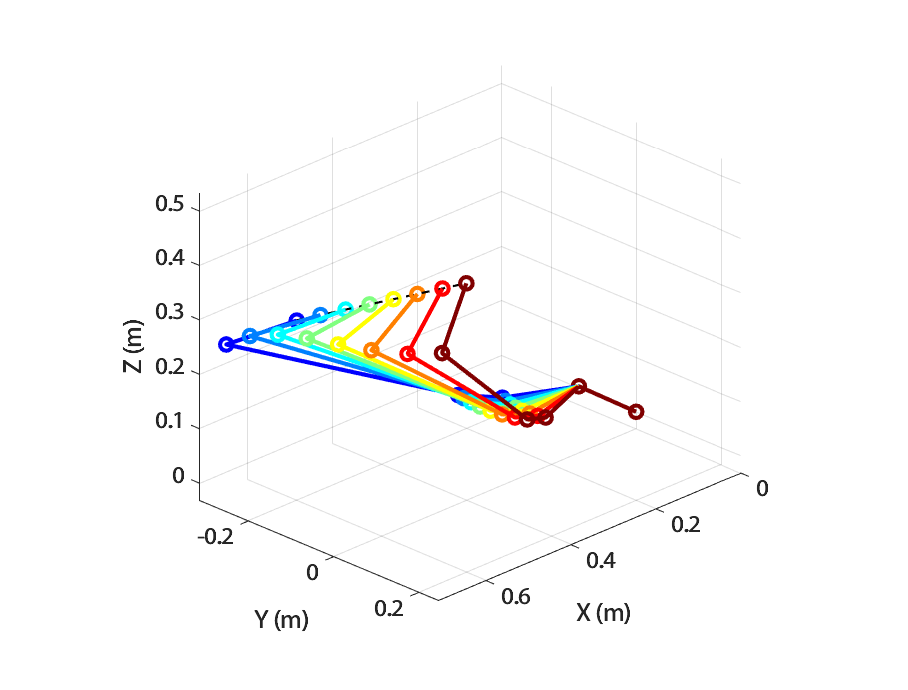
\includegraphics[width =\textwidth]{figures/直线直线.eps}
        }% 这里写第一张图的英文描述
    \end{minipage}
    % \hfill % 撑开左右间距
    % 第二张子图
    \begin{minipage}{0.45\textwidth}
        \centering
        \subfigure[圆弧路径]{\label{fig45:sub2}
            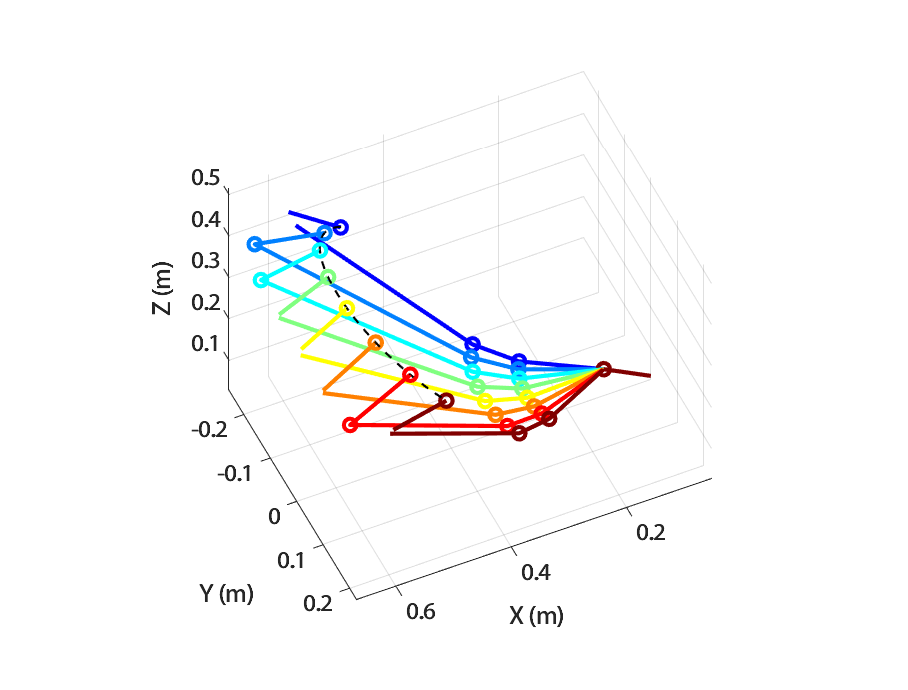
\includegraphics[width =\textwidth]{figures/圆弧圆弧.eps}
        } % 这里写第二张图的英文描述
             % 第一张子图
            \end{minipage}
    % 中英文总标题
    \caption{仿真结果}
    \vspace{-0.5cm}
    \label{fig:total_figure45}
  \end{figure}


% \BiSubsection{关节空间响应}{Subsubsection}
(4)关节空间响应


从图 \ref{pic46} 的关节角度与速度曲线可以看出，各关节在运动起点与终点的速度均经过平滑
过渡，角速度曲线连续且无剧烈脉冲。这证明了本文采用的离散化插补能够为底层电机驱动
器提供高质量的输入信号，避免机械震动。


\begin{figure}[htbp]
    \centering
    % 第一张子图
    \begin{minipage}{0.45\textwidth}
        \centering
        \subfigure[直线路径]{\label{fig45:sub1}
            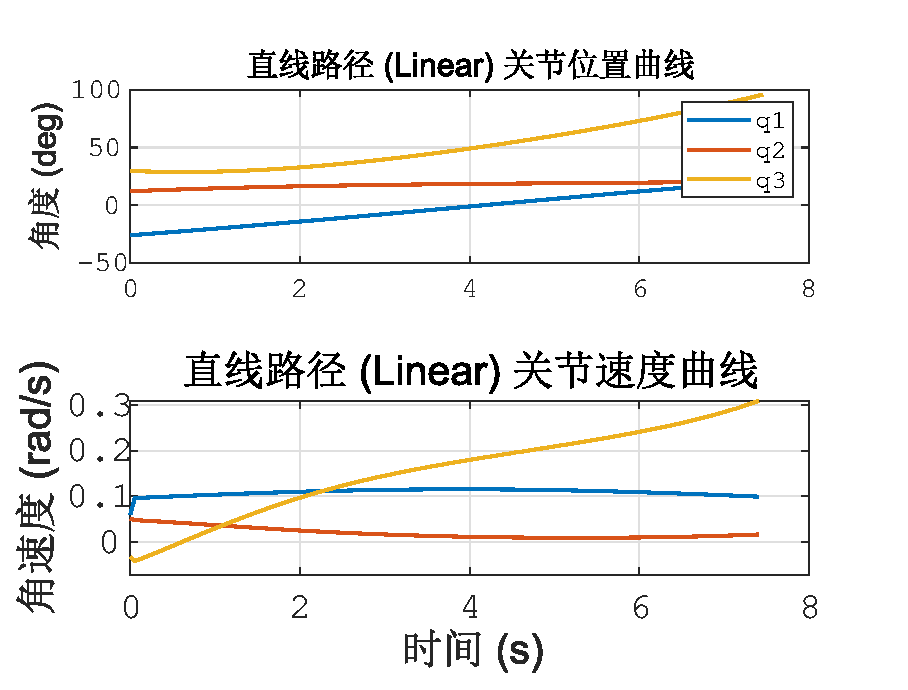
\includegraphics[width =1.1\textwidth]{figures/直线111.eps}
        }% 这里写第一张图的英文描述
    \end{minipage}
    % \hfill % 撑开左右间距
    % 第二张子图
    \begin{minipage}{0.45\textwidth}
        \centering
        \subfigure[圆弧路径]{\label{fig45:sub2}
            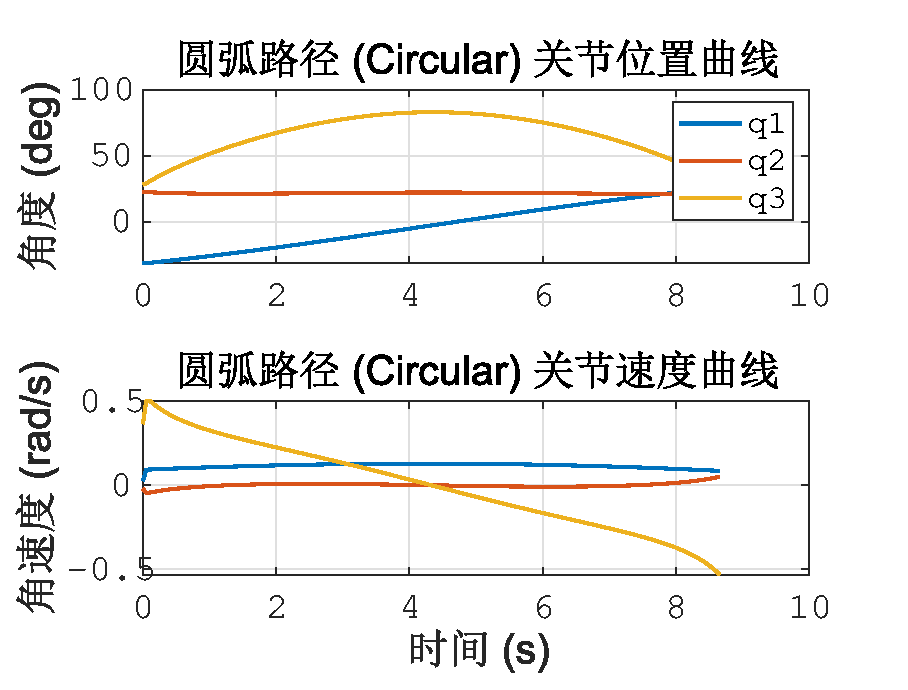
\includegraphics[width = 1.1\textwidth]{figures/圆弧111.eps}
        } % 这里写第二张图的英文描述
             % 第一张子图
            \end{minipage}
    % 中英文总标题
    \caption{关节角度与速度曲线}
    \vspace{-0.5cm}
    \label{pic46}
  \end{figure}
% \BiSubsection{跟踪精度评价}{Subsubsection}
(5)跟踪精度评价



\begin{figure}[H]
    \centering
    % 第一张子图
    \begin{minipage}{0.45\textwidth}
        \centering
        \subfigure[直线路径]{\label{fig46:sub1}
            \includegraphics[width =0.9\textwidth]{figures/直线精度1.eps}
        }% 这里写第一张图的英文描述
    \end{minipage}
    % \hfill % 撑开左右间距
    % 第二张子图
    \begin{minipage}{0.45\textwidth}
        \centering
        \subfigure[圆弧路径]{\label{fig46:sub2}
            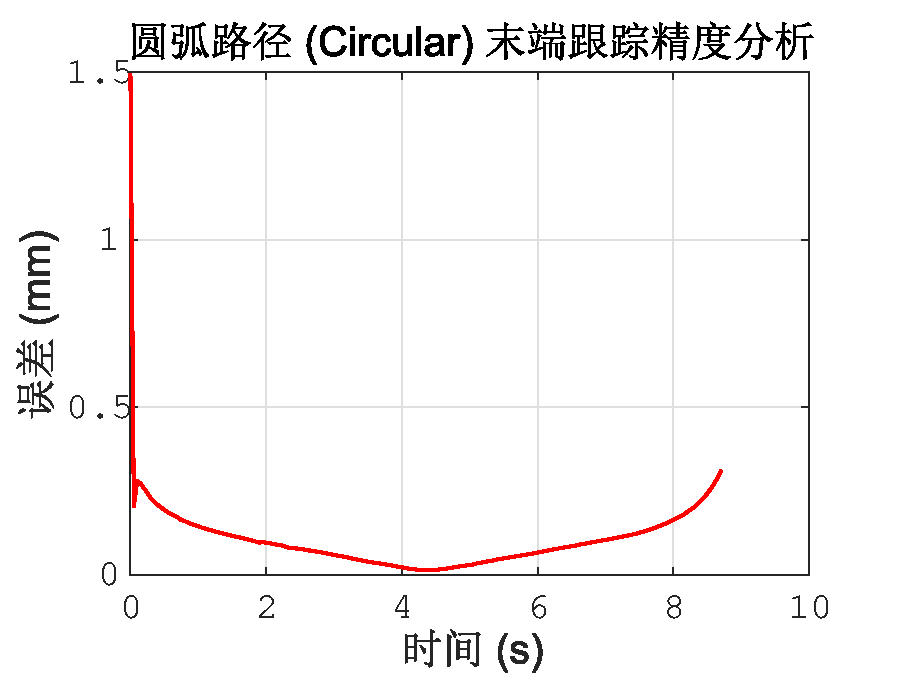
\includegraphics[width = 0.9\textwidth]{figures/圆弧精度11.eps}
        } % 这里写第二张图的英文描述
             % 第一张子图
            \end{minipage}
    % 中英文总标题
    \caption{末端跟踪精度}
    \vspace{-0.5cm}
    \label{pic47}
  \end{figure}


针对空间轨迹，本文算法表现出了极高的跟踪精度。如图 \ref{pic47} 所示，末端执行器在整
个运动周期内的欧氏距离误差保持在 $10^{-1}$mm 量级。






\BiSection{本章小结}{Summary of Chapter}
本章围绕水下绳驱机械臂的运动学建模展开系统研究。
首先，针对传统 D-H 法在平行关节轴线处存在的奇异问题，
采用改进 D-H 法为机械臂建立了连杆坐标系，给出了各关节的几何参数与运动范围，
并通过推导齐次变换矩阵获得了末端位姿关于关节变量的解析表达式，
为后续分析提供了正运动学基础。考虑到绳驱结构耦合关系复杂、
解析解难以直接求取，
文中选用牛顿-拉夫逊数值迭代法实现从期望末端位姿到关节角度的逆运动学求解，
同时深入分析了驱动绳的运动耦合现象，
建立了电机转角与关节转角之间的映射关系，
从而为底层驱动控制提供了直接依据。
在 MATLAB 环境下对逆运动学算法进行了仿真验证，结果表明，
对于工作空间内的目标点，关节角度的迭代求解误差可控制在 0.05\% 以内，
算法精度与收敛性均满足要求。本章建立的模型和求解方法为后续的轨迹规划、
动力学分析以及水下精细控制奠定了必要的理论基础。
\clearpage{
    \pagestyle{plain}
    \cleardoublepage
  }